\documentclass[greek]{beamer}
%\usepackage{fontspec}
\usepackage{amsmath,amsthm}
\usepackage{unicode-math}
\usepackage{xltxtra}
\usepackage{graphicx}
\usetheme{Berlin}
\usecolortheme{seahorse}
\usepackage{hyperref}
\usepackage{ulem}
\usepackage{xgreek}
\usepackage{pgfpages}
%\setbeameroption{show notes on second screen}
%\setbeameroption{show only notes}

\setsansfont{DejaVu Sans}

% \newtheorem{definition}{Ορισμός}

\title{Συναρτήσεις}
\subtitle{Μονοτονία}
\author[Λόλας]{Κωνσταντίνος. Λόλας}
\date{}

\begin{document}

\begin{frame}
 \titlepage
\end{frame}

\section{Θεωρία}
\begin{frame}{Αντίστροφη}
 \begin{block}{Ορισμός}
  Έστω συνάρτηση  $f:Α\to B$ που είναι 1-1. Η αντίστροφή της $f^{-1}:Β\to Α$ ορίζεται η συνάρτηση που για κάθε $x\in f(Α)$ αντιστοιχεί ένα $y\in Α$ ώστε:
  $$f^{-1}(x)=y \iff f(y)=x$$
 \end{block} \pause
 Και επειδή συνήθως το $x$ αφορά το $D_f$
\end{frame}

\begin{frame}{Αντίστροφη}
 \begin{block}{Ορισμός}
  Έστω συνάρτηση  $f:Α\to B$ που είναι 1-1. Η αντίστροφή της $f^{-1}:Β\to Α$ ορίζεται η συνάρτηση που για κάθε $y\in f(Α)$ αντιστοιχεί ένα $x\in Α$ ώστε:
  $$f^{-1}(y)=x \iff f(x)=y$$
 \end{block}

 \centering
 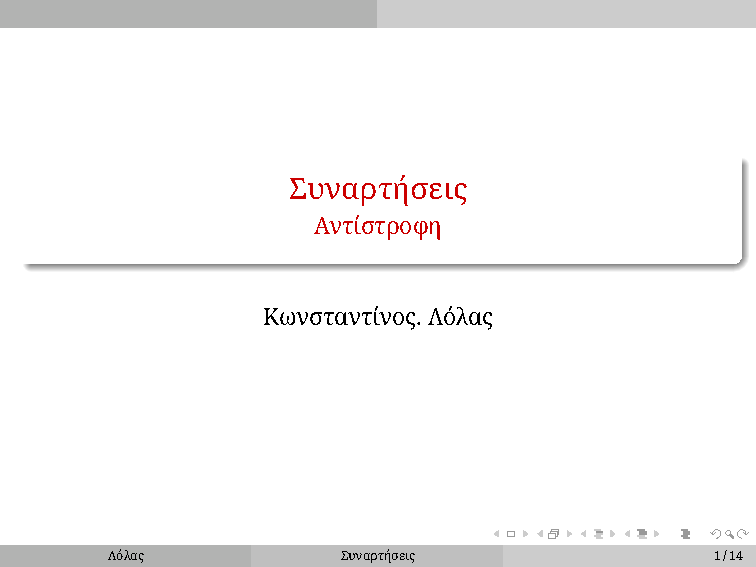
\includegraphics[width=0.35\textwidth]{"images/1.3.4 Μονοτονία.png"}
\end{frame}

\begin{frame}{Μήπως τα έχετε ξαναδεί?}
 \begin{itemize}
  \item $f(x)=x+3$ \pause
  \item $f(x)=2x$ \pause
  \item $f(x)=\sqrt{x}$ \pause
  \item $f(x)=e^x$ \pause
  \item $f(x)=x^2$!!! \pause
  \item Πιο σύνθετες?
 \end{itemize}
\end{frame}

\begin{frame}{Ικανότητες?}
 Τι προσπαθούμε να κάνουμε? \pause
 \begin{itemize}
  \item Να βρίσκουμε από πού ήρθαμε, το $x$! \pause
  \item Σύνολο τιμών
 \end{itemize}
\end{frame}

\begin{frame}{Πώς θα το κάνουμε?}
 Έχετε $y$ και ζητάτε $x$ \pause
 \begin{itemize}
  \item $y=x+3$ \pause
  \item $y=2x$ \pause
  \item $y=\sqrt{x}$ \pause
  \item $y=e^x$ \pause
  \item $y=x^2$!!! \pause
  \item Πιο σύνθετες?
 \end{itemize}
\end{frame}

\begin{frame}{Μπορώ?}
 Σχεδιάστε γραφικά μια 1-1 συνάρτηση. \pause

 Ξέροντας ότι τα $x$ γίνονται $y$ σχηματίστε την $f^{-1}$ \pause

 Άρα:
 \begin{itemize}
  \item Η $f^{-1}$ είναι συμμετρική της $f$ ως προς την ευθεία $y=x$ \pause
  \item Αν η $f$ περνά από την ευθεία $y=x$ τότε και η $f^{-1}$ περνά, και αντίστροφα.
 \end{itemize} \pause
 \begin{alertblock}{Προσοχή στα spam}
  Σχεδιάστε συνάρτηση που δεν έχει μόνο στην $y=x$ κοινά σημεία με την αντίστροφή της.
 \end{alertblock}
\end{frame}

\begin{frame}{Βασική Ιδιότητα}
 \begin{exampleblock}{Κρατηθείτε!}
  \begin{itemize}
   \item $f\left(f^{-1}(x)\right)=x$, για κάθε $x\in f(D_f)$ \pause
   \item $f^{-1}\left(f(x)\right)=x$, για κάθε $x\in D_f$
  \end{itemize}
 \end{exampleblock}
\end{frame}

\section{Ασκήσεις}
\begin{frame}{Εξάσκηση}
 Δίνεται η συνάρτηση $f(x)=e^x-1$
 \begin{enumerate}
  \item Να δείξετε ότι είναι 1-1. \pause
  \item Να δείξετε ότι αντιστρέφεται και να βρείτε την $f^{-1}$
 \end{enumerate}
\end{frame}

\begin{frame}{Εξάσκηση}
 Δίνεται η συνάρτηση $f(x)=\frac{x+4}{x+1}$.
 \begin{enumerate}
  \item Να δείξετε ότι η $f$ είναι συνάρτηση 1-1 \pause
  \item Να βρείτε την $f^{-1}$
  \item Να βρείτε τα κοινά σημεία των $C_f$ και $C_{f^{-1}}$ με τον άξονα συμμετρίας τους.
 \end{enumerate}
\end{frame}

\begin{frame}{Εξάσκηση}
 Δίνεται η συνάρτηση $f(x)=\frac{e^x-1}{e^x+1}$.
 \begin{enumerate}
  \item Να δείξετε ότι η $f$ αντιστρέφεται\pause
  \item Να βρείτε την $f^{-1}$
 \end{enumerate}
\end{frame}

\begin{frame}{Εξάσκηση}
 Έστω $f:[1,+\infty)\to \mathbb{R}$ μία συνάρτηση με $f(x)=(x-1)^2+2$.
 \begin{enumerate}
  \item Να δείξετε ότι η $f$ αντιστρέφεται \pause
  \item Να βρείτε την αντίστροφη της $f$ \pause
  \item Να σχεδιάσετε τις $C_f$ και $C_{f^{-1}}$ στο ίδιο σύστημα αξόνων\pause
  \item Για κάθε $x\ge 1$ θεωρούμε τα σημεία $Α(x,f(x))$ και $Β(f(x),x)$ των $C_f$ και $C_{f^{-1}}$ αντίστοιχα. Να βρείτε την ελάχιστη απόσταση $d$ των σημείων $Α$ και $Β$.
 \end{enumerate}
\end{frame}

\begin{frame}{Εξάσκηση}
 Δίνεται η συνάρτηση $f(x)=x^3$. Να δείξετε ότι η $f$ αντιστρέφεται και να βρείτε την αντίστροφή της.
\end{frame}

\begin{frame}{Εξάσκηση}
 Δίνεται η συνάρτηση $f(x)=\begin{cases}
   \frac{1}{x}, & x<0    \\
   x^2,         & x\ge 0
  \end{cases}$.

 Να δείξετε ότι η $f$ αντιστρέφεται και να βρείτε την $f^{-1}$
\end{frame}

\begin{frame}{Εξάσκηση}
 Έστω $f:\mathbb{R}\to\mathbb{R}$ μία συνάρτηση, με $f(\mathbb{R})=\mathbb{R}$, η οποία ικανοποιεί την σχέση
 $$f^3(x)+f(x)-x-1=0\text{, για κάθε }x\in \mathbb{R}$$
 \begin{enumerate}
  \item Να δείξετε ότι η $f$ αντιστρέφεται και να βρείτε τη συνάρτηση $f^{-1}$ \pause
  \item Να βρείτε τα κοινά σημεία της $C_f$ και της ευθείας $y=x$
 \end{enumerate}
\end{frame}

\begin{frame}{Εξάσκηση}
 Δίνεται η συνάρτηση $f(x)=x^5+x$, με $f(\mathbb{R})=\mathbb{R}$
 \begin{enumerate}
  \item Να δείξετε ότι η $f$ η $f$ αντιστρέφεται \pause
  \item Να βρείτε τα κοινά σημεία των $C_f$ και $C_f^{-1}$
 \end{enumerate}
\end{frame}

\begin{frame}{Εξάσκηση}
 Έστω $f:\mathbb{R}\to\mathbb{R}$ μία συνάρτηση, με $f(\mathbb{R})=\mathbb{R}$, η οποία είναι γνησίως φθίνουσα και $f(0)=1$, $f(1)=-2$.
 \begin{enumerate}
  \item Να δείξετε ότι η $f$ η $f$ αντιστρέφεται \pause
  \item Να βρείτε τις ρίζες και το πρόσημο της $f^{-1}$ \pause
  \item Να λύσετε την εξίσωση $f\left(f^{-1}(3x+4)-f^{-1}(-2)\right)=1$ \pause
  \item Να λύσετε την ανίσωση $f^{-1}\left(3+f(\ln x)\right)>0$
 \end{enumerate}
\end{frame}

\begin{frame}{Εξάσκηση}
 Έστω $f:\mathbb{R}\to\mathbb{R}$ μία συνάρτηση, με $f(\mathbb{R})=\mathbb{R}$, η οποία είναι γνησίως αύξουσα.
 \begin{enumerate}
  \item Να δείξετε ότι η $f$ η $f$ αντιστρέφεται και $f^{-1}\uparrow$\pause
  \item Αν η $f$ είναι περιττή, να αποδείξετε ότι και η $f^{-1}$ είναι περιττή \pause
  \item Αν ισχύει $f(x)>x$ για κάθε $x\in\mathbb{R}$, να δείξετε ότι
        $$f^{-1}(x)<x\text{, για κάθε }x\in\mathbb{R}$$
 \end{enumerate}
\end{frame}

\begin{frame}{Εξάσκηση}
 Έστω $f:\mathbb{R}\to\mathbb{R}$ μία συνάρτηση, με $f(\mathbb{R})=\mathbb{R}$, η οποία είναι γνησίως φθίνουσα και $f(0)=1$.
 \begin{enumerate}
  \item Να δείξετε ότι η $f$ η $f$ αντιστρέφεται \pause
  \item Να λύσετε την ανίσωση $f(x)-f^{-1}(1-x)<x+1$
 \end{enumerate}
\end{frame}

\begin{frame}
 Στο moodle θα βρείτε τις ασκήσεις που πρέπει να κάνετε, όπως και αυτή τη παρουσίαση
\end{frame}

\end{document}
